\begin{figure*}[t]
\centering
{\small
\begin{tikzpicture}[
    node distance=1.5cm and 1.8cm,
    block/.style={rectangle, draw=blue!80!black, fill=blue!60, text=white, text width=2.5cm, align=center, minimum height=1cm, font=\bfseries},
    lbl/.style={rectangle, draw=black, thick, fill=white, text=black, text width=2.2cm, align=center, font=\bfseries\footnotesize, minimum height=1cm},
    arrow/.style={-{Latex[width=2mm]}, thick, black},
    arrowlabel/.style={font=\bfseries\footnotesize, text=black, midway, above},
    bluearrow/.style={-{Latex[width=2mm]}, thick, blue!80!black},
    bluearrowlabel/.style={font=\bfseries\footnotesize, text=blue!80!black, midway, below}
]

% Top row - main black border + white fill boxes with black text
\node[lbl, xshift=-1.5cm] (C21a) {Chapter 4\\Entanglement Aware\\Tether Planner};
\node[lbl, right=of C21a] (C21b) {Chapter 5\\Visual Tracking\\NMPC};
\node[lbl, right=of C21b] (C1) {Chapter 3\\Underwater Robot\\Simulator};

% Second row - vertically aligned blocks under their top boxes with smaller shift
\node[block, below=of C21a, xshift=-0.3cm] (PathPlanner) {Path Planner};
\node[block, below=of C21b, yshift=-2pt] (Cost) {Cost};

\node[font=\bfseries\itshape\large] at ($(Cost.north)+(0.7cm,0.75cm)$) {MPC};




% Image node larger
\node[below=of C1] (Sim) {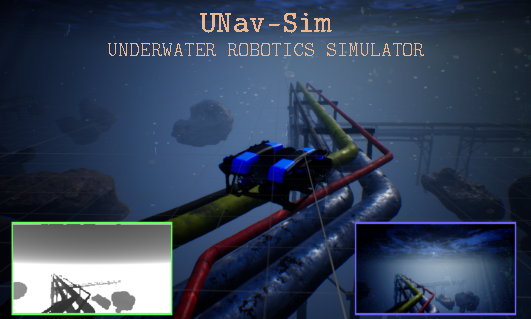
\includegraphics[width=4.0cm]{Phd_thesis/figures/UWRS_pipe.pdf}};

% Third row - filled blue blocks with white text
\node[block, below=of PathPlanner] (Model) {Model};
\node[block, below=of Cost] (Optimizer) {Optimizer};

% Bottom row - black border + white fill boxes with black text
\node[lbl, below left=0.8cm and -0.5cm of Model] (C31) {Chapter 6\\Full Model\\(PINNS)};
\node[lbl, below right=0.8cm and -0.5cm of Model] (C32) {Chapter 7\\Residual Model\\(GPs)};

% Connections from top black boxes
\draw[arrow] (C21a.south) -- ++(0,-1.5cm);
\draw[arrow] (C21b) -- (Cost);
\draw[arrow] (C1) -- (Sim);

% Main process flow
\draw[arrow] (PathPlanner) -- node[arrowlabel, xshift=-0.1cm] {reference} (Cost);

\coordinate (arrowStart) at ($(Cost.east) + (0.5,0)$);
\draw[arrow, blue] (arrowStart) -- (Cost.east);
\draw[thick, blue] (arrowStart) -- ++(0,-0.9);

\draw[arrow] (Model) -- node[arrowlabel] {prediction} (Optimizer);

% Model learning connections
\draw[arrow] (C31) -- (Model);
\draw[arrow] (C32) -- (Model);

% New connection from image to Model (feedback) in blue
\draw[bluearrow] 
  ([xshift=2mm]Sim.west) -- % shifted starting point 2mm to the right
  node[bluearrowlabel, xshift=2cm] {feedback} ++(-6.86,0)
  -- ++(0,-1)
  -- (Model.north);

% New arrow from Optimizer: right 3cm then up 0.5cm
\draw[arrow, line width=1.6pt]
  (Cost.south) -- node[arrowlabel, left] {performance metric} ++(0,-1.5cm);

\draw[arrow] (Optimizer.east) -- node[arrowlabel, below] {actions} ++(3,0) -- ++(0,0.5);

\begin{scope}[on background layer]
    % Coordinates for the 6 corners of the L-shaped polygon
    \coordinate (A) at ([xshift=-0.3cm,yshift=0.5cm]Cost.north west);
    \coordinate (B) at ([xshift=0.3cm,yshift=3.cm]Optimizer.north east);
    \coordinate (C) at ([xshift=0.3cm,yshift=-0.5cm]Optimizer.south east);
    \coordinate (D) at ([xshift=-3cm,yshift=-.5cm]Model.south east);
    \coordinate (E) at ([xshift=-0.3cm,yshift=2.07cm]Model.south west);
    \coordinate (F) at ([xshift=-0.3cm,yshift=-0.5cm]Cost.south west);
    
    % Draw enclosed 6-sided dashed box
    \draw[dashed, thick]
        (A) -- (B) -- (C) -- (D) -- (E) -- (F) -- cycle;
\end{scope}

\end{tikzpicture}
}
\caption{Block diagram illustrating the underwater robot planning and control components with their connections. Blue blocks indicate key process modules (Path Planner, Cost, Model, Optimizer), while top and bottom boxes represent related components with black borders and white fill. Feedback from the simulator image is integrated into the model learning process.}
\label{fig:uw_robot_planning_control}
\end{figure*} 